The diffraction condition in the case of a three-dimensional regular grating with elastic scattering takes the form~\cite{Kittel86}:

    \begin{equation}
        \begin{cases}
        \begin{aligned}
            \left( \vectbf{D}{x},\: \vectbf{e}{\textrm{out}} - \vectbf{e}{\textrm{in}}\right) &= h \lambda
            \\
            \left( \vectbf{D}{y},\: \vectbf{e}{\textrm{out}} - \vectbf{e}{\textrm{in}}\right) &= k \lambda
            \\
            \left( \vectbf{D}{z},\: \vectbf{e}{\textrm{out}} - \vectbf{e}{\textrm{in}}\right) &= l \lambda
        \end{aligned}
        \end{cases}
        \label{bragg_wolf_order}
    \end{equation}
    \begin{equation*}
    \end{equation*}

\noindent where $h,\:k,\:l$ are Miller indices represented by integers, $\vectbf{D}{i}$ is a vector connecting adjacent lattice nodes along the $i$ direction, $\vectbf {e}{\textrm{in}}$ is the unit vector of the direction of the incident radiation, $\vectbf{e}{\textrm{out}}$ is the unit vector of the direction of the transmitted radiation. Passing to spherical coordinates related to $\vectbf{e}{\textrm{in}}$ so that in Cartesian representation $\vectbf{e}{\textrm{in}} = \vectbf{e}{z}$ , \ref{bragg_wolf_order} can be converted as follows, given that $|\vectbf{D}{x}| = |\vectbf{D}{y}| = |\vectbf{D}{z}| = d$ for the considered cubic lattice:

    \begin{equation}
        \begin{cases}
            \cos{\theta_0}\sin{\Delta \theta}\cos{\left( \Delta \varphi - \varphi_0 \right)} - \sin{\theta_0} \left( \cos{\Delta \theta} - 1 \right) = \cfrac{h^{\prime} \lambda}{d}
            \\
            \sin{\Delta \theta} \sin{\left( \Delta \varphi - \varphi_0 \right)} = \cfrac{k^{\prime} \lambda}{d}
            \\
            \sin{\theta_0}\sin{\Delta \theta}\cos{\left( \Delta \varphi - \varphi_0 \right)} + \cos{\theta_0} \left( \cos{\Delta \theta} - 1 \right)= \cfrac{l^{\prime} \lambda}{d}
        \end{cases}
        \label{bragg_wolf_order_spherical}
    \end{equation}
    \begin{equation*}
    \end{equation*}

\noindent where $\Delta \theta,\:\Delta \varphi$ are the angles characterizing the deviation of the direction of the diffracted radiation relative to the incident one, $\theta_0,\:\varphi_0$ are the angles characterizing the rotation of the target (grid) in space , $h^\prime,\:k^\prime,\:l^\prime$ --- new Miller indices (\ref{3ddiffr:image}). Using \ref{bragg_wolf_order_spherical}, we can obtain the angular distribution of diffracted radiation for given initial parameters $d$, $\lambda$, $\theta_0$, $\varphi_0$.

\begin{tikzfigure}
    \subcaptionbox{$xz$ projection.}{
        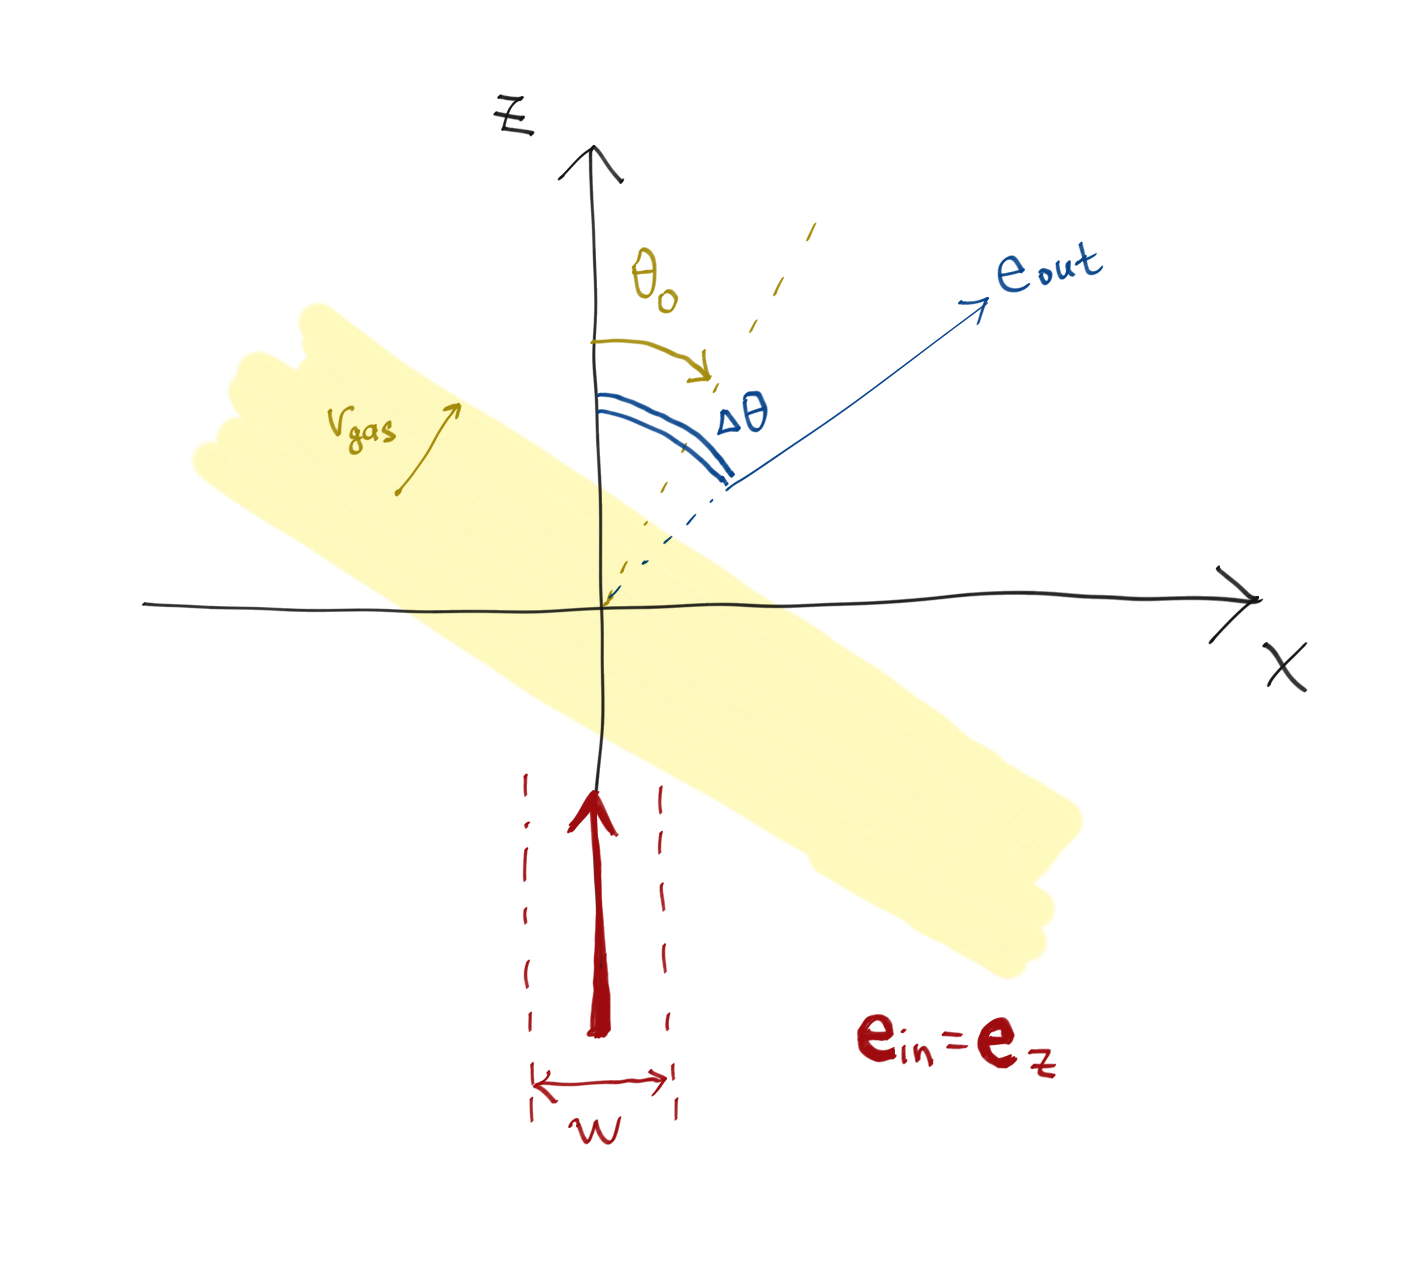
\includegraphics[width=0.45\linewidth]{../components/img/3ddiffrxzgas}
    }
    \hfil
    \subcaptionbox{$xy$ projection.}{
        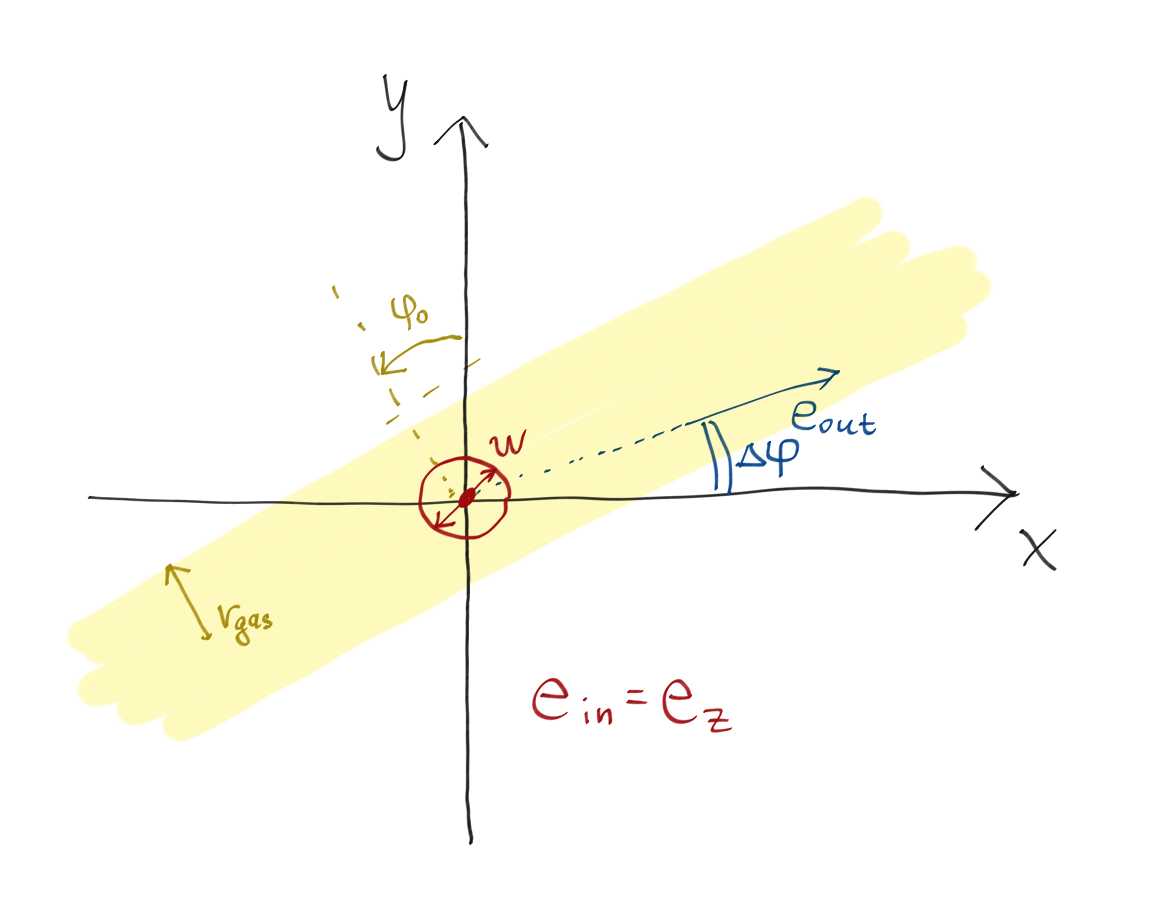
\includegraphics[width=0.45\linewidth]{../components/img/3ddiffrxygas}
    }
    \label{3ddiffr:image}\caption{General scheme of interaction of incident radiation with a grating. $\theta_0$, $\varphi_0$ --- characterize the target angles in space, $\Delta \theta$, $\Delta \varphi$ --- angles of deflection of the direction of the diffracted radiation relative to the incident, $r_{\textrm{gas }}$ is the radius of the gas jet representing the target, $w$ is the diameter of the Gaussian beam of incident radiation. $\Delta \theta$ is counted counterclockwise around $y$, $\Delta \varphi$ --- counterclockwise around $z$.}
\end{tikzfigure}

% \begin{figure}[H]
%     \subimgtwo[components/img/3ddiffrxzgas]{Проекция на плоскость $xz$.}{3ddiffr:a}{0.4\textwidth}
%     \hfil
%     \subimgtwo[components/img/3ddiffrxygas]{Проекция на плоскость $xy$.}{3ddiffr:b}{0.4\textwidth}
%     \caption{Общая схема взаимодействия падающего излучения с решеткой. $\theta_0$, $\varphi_0$ --- характеризуют углы покорота мишени в пространстве, $\Delta \theta$, $\Delta \varphi$ --- углы отклонения направления дифрагировавшего излучения относительно падающего, $r_{\textrm{gas}}$ --- радиус газовой струи, представляюшей мишень, $w$ --- диаметр гауссова пучка падающего излучения. $\Delta \theta$ отсчитывается вокруг $y$ против часовой стрелки, $\Delta \varphi$ --- вокруг $z$ против часовой стрелки.}\label{3ddiffr:image}
% \end{figure}